\documentclass{article}
%Para imagenes
\usepackage{graphicx}
\usepackage{float}
\usepackage{enumitem} % Paquete para personalizar listas
\usepackage[margin=2cm]{geometry} % Ajusta todos los márgenes a 2 centímetros
\usepackage{indentfirst} % Este paquete fuerza la sangría del párrafo en la primera línea
\setlength{\parindent}{1cm} % Ajusta la sangría de los párrafos a 1 cm


\begin{document}
    \begin{titlepage}
        \centering
        {\bfseries\LARGE Universidad de Granada\par}
        \vspace{1cm}
        {\scshape\Large Facultad de Ingeniería Informática \par}
        \vspace{2cm}
        {\scshape\Huge Practica 2: Diseño adaptativo en Flutter \par}
        \begin{figure}[h]
                \centering
                
\includegraphics[width=0.6\textwidth]{logo_UGR.jpg}
                \label{fig:portada}
            \end{figure}
        {\itshape\Large DS: Grupo 1.7\par}
        \vfill
            {\Large  Emanuel Giraldo Herrera\par}
            {\Large  Thomas Lang \par}
            {\Large  Timur Sorokin \par}
            {\Large  Alejando Iborra Morán \par}
        \vfill
        {\Large (2023-2024) \par}
    \end{titlepage}

\tableofcontents

\newpage
\section{Abstract}

En este documento se detalla el proceso de adaptación del ejercicio 3 de la práctica 1 desarrollado en Java al nuevo framework denominado Flutter.
La tarea principal consistió en realizar el mantenimiento adaptativo y perfectivo de modo que se ha migrado de un lenguaje a otro y se añadido una interfaz gráfica para 
permitir la interacción del usuario con el sistema.

Durante el proceso de migración a Dart nos hemos encontrado con las diferencias fundamentales entre los dos lenguajes como es el caso de sintaxis y el manejo de valores NULL.

En cuanto al diseño de la interfaz de usuario (UI), se priorizó la funcionalidad sobre la estética, ya que nuestro objetivo consistia en presentar un prototipo que permitiera mostrar 
la interacción del usuario con el sistema. De modo que la interfaz se diseñó de manera sencilla y eficiente, centrándose sobretodo en la usabilidad y la claridad de la información presentada.

Finalmente, el resultado obtenido fue una pequeña aplicación que permite al usuario crear personajes seleccionando diferentes opciones y muestra los datos del personaje creado.


\section{Introducción}

En esta práctica se ha introducido un nuevo framework llamado Flutter desarrollado por Google. Este ofrece una serie de herramientas a los desarrolladores para 
crear aplicación multiplataforma con una sola base de código, es decir, el desarrollador escribe el código una vez y este puede ser compilado para diferentes plataformas como linux, windows, ios y android.

El concepto esencial de Flutter son los widgets, los cuales representan los componentes visuales de la aplicación. 
Estos widgets son altamente personalizables y pueden ser extendidos con facilidad, lo que permite a los desarrolladores crear interfaces
de usuario de manera rápida y eficiente para múltiples plataformas. Este enfoque no solo agiliza el proceso de desarrollo, sino que también 
reduce los costos asociados con el mantenimiento de aplicaciones para diferentes plataformas.

Sin embargo, a pesar de sus beneficios, Flutter también presenta algunas desventajas que deben ser consideradas:

\begin{itemize}
\item - Curva de aprendizaje: Para los desarrolladores nuevos en Flutter, puede haber una curva de aprendizaje significativa, especialmente si no están familiarizados con el paradigma de desarrollo basado en widgets.
\item - Legibilidad del código con widgets anidados: En los casos donde se utilizan múltiples widgets anidados la legibilidad del código disminuy drasticamente dificultando el mantenimiento y la comprensión del código.
\item - Tamaño de la aplicación más grande: Debido a la inclusión del motor de Flutter y otros recursos necesarios en cada aplicación, el tamaño del ejecutable compilado suele ser más grande en comparación con las aplicaciones nativas.
\item - SetState repinta todos los elementos: En Flutter, el uso de la función setState() para actualizar el estado de un widget provoca que todos los elementos se vuelvan a pintar, lo que puede afectar el rendimiento de la aplicación en casos de actualizaciones frecuentes del estado.
\end{itemize}

A modo de conclusión podemos decir que a pesar de las desventajas mencionadas Flutter sigue siendo una opción relevante en el entorno de desarrollo crossplatform. Además, siendo un proyecto
respaldado por Google da cierta garantia y seguridad en cuanto al futuro de este. 

\subsection{Análisis del problema}
A partir de la información expuesta en el guion de la practica se identifican claramente las siguientes dos propuestas:

    \begin{itemize}
        \item 1. Realizar el mantenimiento adaptativo:

        Esta fase se realiza la migración del código existente en Java, obtenido en prácticas anteriores, al lenguaje Dart. El objetivo es adaptar el código para que sea compatible con el nuevo framework Flutter. 

        \item 2. Realizar el mantenimiento perfectivo:

        En esta etapa se introduce un nuevo componente al sistema que es una interfaz de usuario (UI). Para ello recurimos al uso de los Widgets que nos permiten crear componentes visuales de la aplicación.
        Se han considerado los aspectos tales como la navegación entre pantallas, la disposición de los elementos de la interfaz y la respuesta a las acciones del usuario. 
    \end{itemize}

\section{Desarrollo}

\subsection{Fase 1: Migración a Dart}

Para afrontar la migración del código de un lenguaje a otro, hemos dedicado un tiempo para familiarizarnos con la sintaxis de Dart. Gracias a los ejercicios indivuales propuestos tuvimos oportunidad de obtener un poco de experiencia en el manejo de este lenguaje. Dada la simplicidad de este proceso, no consideramos necesario profundizar en detalles específicos.

Posteriormente, hemos procedido a revisar la relación entre las entidades del sistema. En particular, hemos prestado especial atención a las clases Fachada y Menú. Dado que en la practica anterior la interacción con el sistema se llevaba a cabo mediante la terminal
era necesario unir los modulos mediante una clase Fachada. No obstante, ahora, puesto que hemos añadido una interfaz grafica (UI) su presencia es dudosa cuanto menos. 

Despues de debatirlo, hemos decidido mantener la estructura previa del código intacta. Esta decisión se basa en la utilidad potencial de la clase Menú como herramienta para la depuración y las pruebas en entornos donde no sea necesaria una interfaz gráfica.


\subsection{Fase 2: UI}



Durante esta fase del proyecto, nos hemos dedicado a revisar la documentación sobre los Widgets en Flutter. Utilizando los recursos disponibles en la página oficial del proyecto, hemos encontrado ejemplos prácticos que han sido de gran ayuda para el desarrollo de esta etapa de la práctica.

Puesto que al tratarse de un proyecto en el campo de la ingeniería software, hemos adoptado un enfoque más practico en cuanto al diseño de la interfaz, priorizando la funcionalidad y claridad sobre consideraciones estéticas. Al final de todo, solo pretendemos mostrar un prototipo que demuestre la interacción entre distintos componentes del sistema.  

Por ultimo, consideramos importante mencionar que la clase CreadorDePersonajes juega un papel clave en la aplicación. Esta clase se encarga de manejar la lógica relacionada con la interacción del usuario y la creación de personajes. En otras palabras, se asemeja al concepto de Controlador en el modelo MVC. 

\subsection{Problemas encontrados}

Durante el desarrollo de la aplicación han sido diversos los problemas encontrados. Entre estos podemos nombrar algunos sin mucha relevancia que aún así impedían el correcto funcionamiento de la aplicación y otros que han supuesto un verdadero dolor de cabeza.


\begin{itemize}
    \item Problema de lectura de los HasMaps:
    
    \hspace{1cm}Las características de los personajes vienen definidas por su clase y raza y se representan en HasMaps que almacenan el nombre del atributo correspondiente y su valor numérico. Estos atributos y sus valores se encuentran en los archivos .txt de cada clase y raza. La idea es leer estos archivos para generar así los HashMaps con las claves y valores específicos.
    
    \hspace{1cm}Para ello en un primer momento se había optado por utilizar openRead() seguido de funciones para separar las líneas y posteriormente iterar en cada una para extraer los datos. Sin embargo, el problema es que no se hacía correctamente la iteración de las líneas por problemas con las funciones que manejaban el archivo.

    \hspace{1cm}Debido a que ese enfoque no ha resultado fructífero en ninguna de sus variantes, hemos decido utilizar otra aproximación usando la función readAsLinesSync(), pudiendo acceder a las líneas del archivo directamente y con la misma idea de iterar en cada una de ellas para extraer los datos.


    \item Errores con la clase Ladrón:

    \hspace{1cm}Con la aplicación aparentemente funcionando de forma correcta, seleccionar la clase Ladrón no devolvía un personaje con dicha clase. Después, de un análisis rápido hemos visto que el problema era utilizar `ladrón', con la tilde correspondiente, como selectedClass en el boton de la clase Ladrón, mientras que el procesamiento en la función \textunderscore{}crearPersonaje() llamaba al LadronBuilder(), solo en el caso de que estuviera seleccionado `ladron', sin tildar. La solución ha sido tan sencilla como unificar la cadena de caracteres en ambos casos a `ladron'.
    
    \item Your CPU does not support required features (VT-x or SVM)
    
    \hspace{1cm} En los dispositivos que no tienen soporte para VT-x (intel) o SVM (amd) resulta imposible emular dispositivos android y de forma transitiva realizar pruebas de ejecución. No obstante, la solución para mitigar esto es cambiar la plataforma de destino. Es decir, ya que flutter es crossplatform podemos compilar ejecutables, por ejemplo, para Linux.  
    
\end{itemize}

\subsection{Widgets utilizados}

\begin{itemize}[label=-]

\item MyApp: 
Se trata de StatelessWidget que define el entry point (main)

\item CreadorDePersonajes: 
Es de tipo StatefulWidget que representa la pantalla principal de la aplicación donde se crea un personaje. 

\item \textunderscore{}CreadorDePersonajes: 
    Se utiliza para representar el estado de la pantalla principal. (raza seleccionada, nombre del personaje...)

\item RaceButton:
    Es un widget sin estado. Encapsula definiciones de estilo para todos los botones de razas (reutilización del código)

\item ClassButton: 
    Misma idea que RaceButton. Se utiliza para no repetir el mismo código.

\item CharacterDetailsScreen: 
    Es un widget sin estado. Se trata de una vista con los detalles del personaje creado.
    

\item buildLineaAtributo:
    Este widget sin estado  se utiliza para construir una línea de atributo en la pantalla de detalles del personaje.

\end{itemize}

\newpage
\section{Ejecución}

\begin{figure}[h]
    \centering
    \vspace{5pt}
    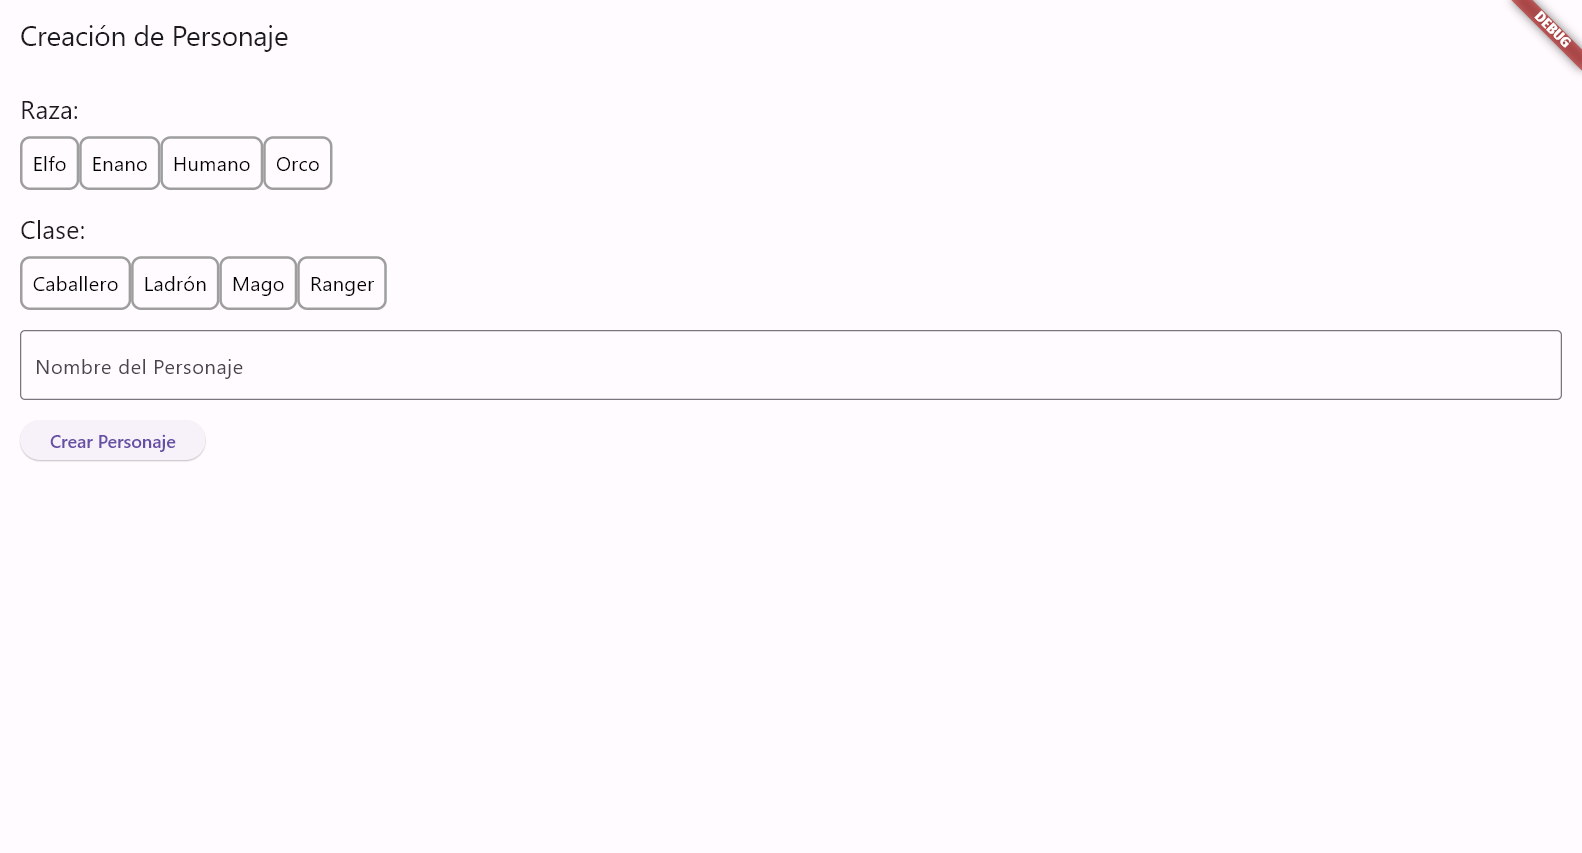
\includegraphics[width=0.9\textwidth]{Ejecucion_1.png}
    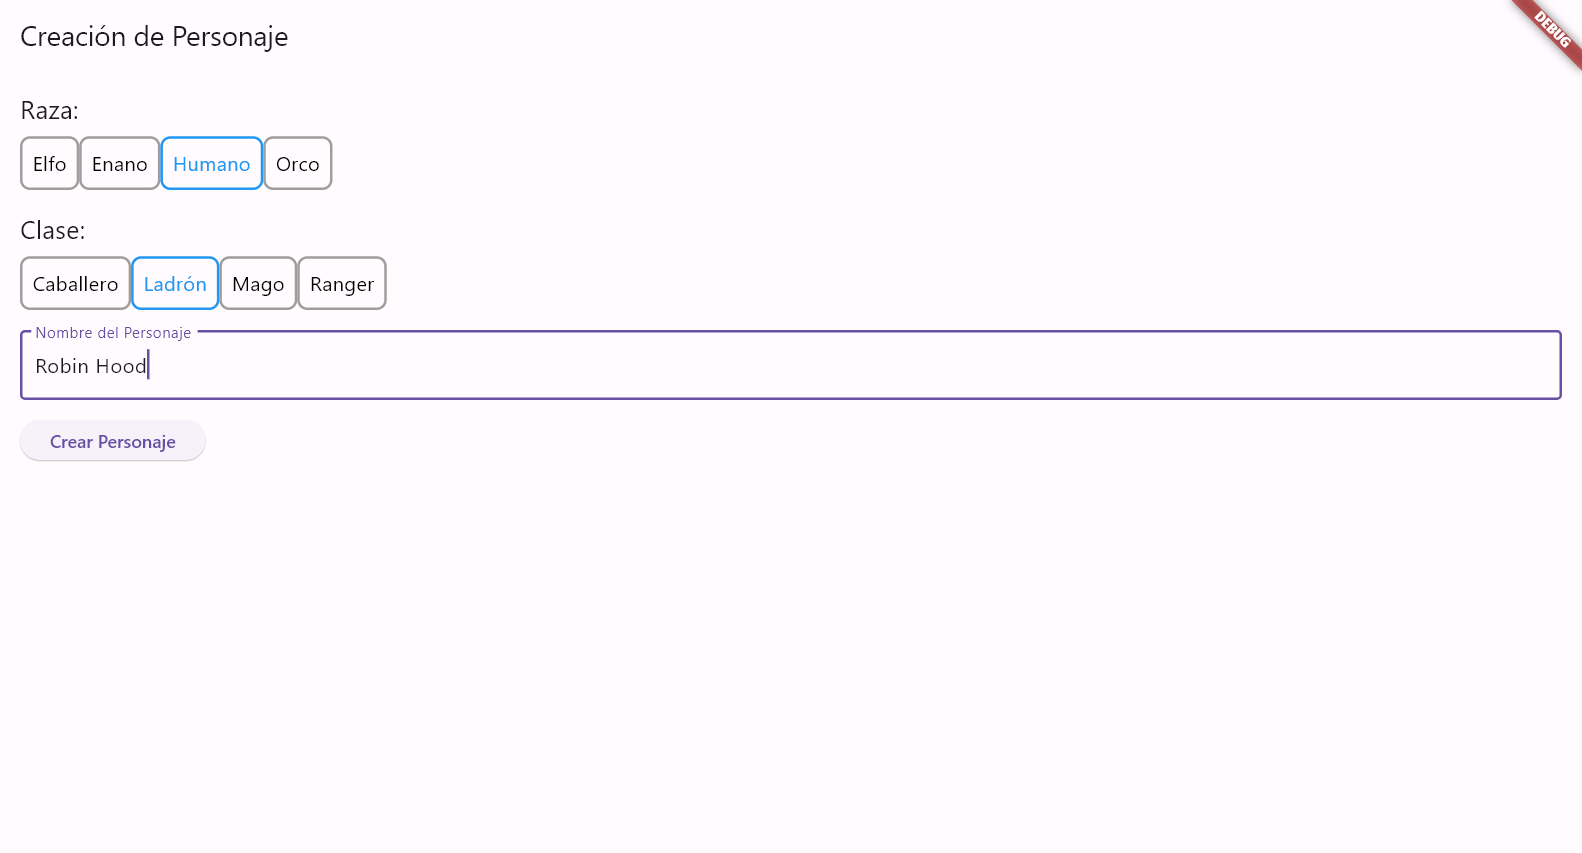
\includegraphics[width=0.9\textwidth]{Ejecucion_2.png}
    \caption{Pantalla de selección de personaje}
    \label{fig:ejecucion_1}
\end{figure}

\begin{figure}[h]
    \centering
    \vspace{5pt}
    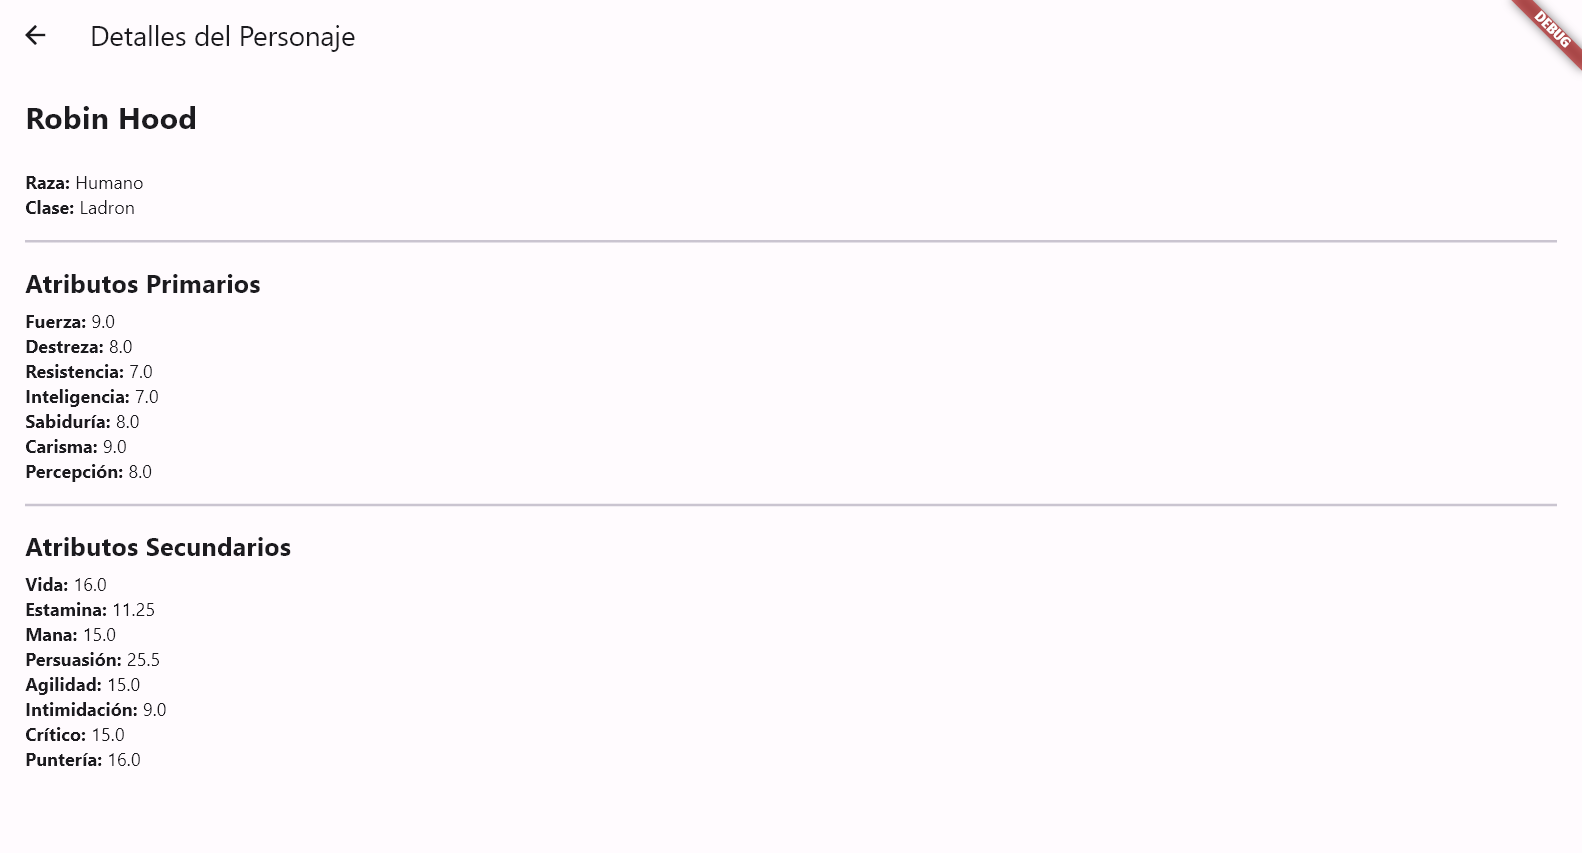
\includegraphics[width=0.9\textwidth]{Ejecucion_3.png}
    \caption{Pantalla de detalle del personaje}
    \label{fig:ejecucion_2}
\end{figure}

\end{document} 